\documentclass[12pt]{extreport}

\usepackage[a4paper, total={6in, 8in}]{geometry}
\usepackage{amsfonts}
\usepackage{amsmath}
\usepackage{amsthm}
\usepackage{hyperref}
\usepackage{tikz}
\usepackage{graphicx}
\usepackage{float}
\usepackage[utf8]{inputenc}
\usepackage{fontenc}
\usepackage[boxruled,linesnumbered]{algorithm2e}
\usepackage{booktabs}
\usepackage{multirow}
\usepackage{adjustbox}
\usepackage{cleveref}
\usepackage[sorting=none, backend=biber]{biblatex}
\usepackage{svg}

%For fun only...
\usepackage{times}

%Bibliographies
\bibliography{references,rfc}

\theoremstyle{plain}
\newtheorem{theorem}{Theorem}[section]
\newtheorem{lemma}[theorem]{Lemma}
\newtheorem{proposition}[theorem]{Proposition}
\newtheorem*{corollary}{Corollary}

\theoremstyle{definition}
\newtheorem{definition}{Definition}[section]
\newtheorem{conjecture}{Conjecture}[section]
\newtheorem{example}{Example}[section]

\theoremstyle{remark}
\newtheorem*{remark}{Remark}
\newtheorem*{note}{Note}

\crefname{algocf}{alg.}{algs.}
\Crefname{algocf}{Algorithm}{Algorithms}

%Title
\title{Some Security Considerations over Contiki-based Sensor Network}
%Authors
\author{Yan Yan}
\date{\today}

\begin{document}

\maketitle

\tableofcontents

%Body
%

\section{Introduction}

Hello, world!

\section{Introduction}
Applications for IoT flourish, leaving a great desire for not only energy efficient, cheap devices, but also for devices that support basic cryptographic functionality such as confidentiality and/or authenticity. Popular algorithms are e.g. the Advanced Encryption Standard\cite{AES} (AES) for confidentiality, and the Elliptic Curve Digital Signature Algorithm\cite{ECDSA} (ECDSA) for authenticity, which, when used in conjunction, enable applications to establish secure end-to-end channels via e.g. Datagram TLS\cite{DTLS} (DTLS). 

However whilst AES is a secure block cipher, one might require randomness to turn it into a secure encryption scheme for arbitrary length messages. Somewhat similarly, ECDSA relies on a known-to-be-secure mathematical problem. However, it also requires large and securely generated random numbers. Consequently, when supporting cryptography the secure generation of random numbers is crucial. 

%The prospering IoT applications constantly proposes higher requirements to security where cryptography plays an important role. Among all prerequisite of implementing cryptographic primitives on these IoT devices, a reliable Random Number Generator (RNG) is critical as it is required in most cryptographic algorithms. In practice, a RNG typically involves a Pseudo Random Number Generator (PRNG) seeded by a high entropy physical source.

In 2013, Texas Instruments (TI) launched a new System-on-chip (SoC), the CC2538\cite{CC2538}, featuring secure channels over 802.15.4 via multiple cryptographic hardware accelerators. Partially because of these cryptographic accelerators, projects such as Contiki\cite{Contiki} and OpenWSN\cite{OpenWSN} began to support the CC2538 with enthusiasm. As of writing this paper, the chip features in the suggested list for Zigbee and 6LoWPAN solutions on TI's website\cite{ZigbeeProducts}.

However, despite all the cryptographic hardware support, the CC2538 does not have a Random Number Generator (RNG) dedicated for cryptographic applications; instead, the user's guide suggests to use a 16 bit Linear Feedback Shift Register (LFSR) as a Pseudo RNG (PRNG) where the seed is generated by the Radio Frequency (RF) module sampling from the radio noise. Whilst the user guide at no point suggested that this method should be used in conjunction with cryptographic algorithms, developers have little choice in the absence of alternatives. Also, in the absence of published attacks, there is often a temptation to ignore warnings towards insecure RNG implementations such as in \cite{SmartMeterBlog}. 

\subsection{Our Contribution}
We show in this study that this choice proves catastrophic for cryptographic applications, not only because the in-built PRNG has only 16 bit entropy which can be easily predicted, but also because we are able to practically demonstrate how to bias the seed obtained from the RF module through the RF interface. Consequently, even if the weak in-built PRNG was replaced by a stronger component, the source for the seed could still be tampered with and thus render the system insecure. All the experimental work in this paper are performed on the latest Contiki release version 3.0.
%The related source code can be accessed at \cite{prngtest}.

Our paper is structured as follows. We begin in \Cref{ContikiDriverIssue} with some Contiki RNG driver issues for CC2538. \Cref{LFSR} revises why using a 16 bit LFSR as PRNG is a bad practice and we show how this design flaw can be exploited to break DTLS in \Cref{BreakDTLS}, before reviewing the problem in \Cref{PRNGReflection}. In \Cref{Seed} we explain how CC2538 samples the radio noise into random seed and then we demonstrate a bias attack in \Cref{Jamming} which could be achieved given physical access to the device. Finally we conclude the paper in \Cref{Conclusion}.

\subsection{Related Work}
The design flaw of using a 16 bit LFSR as PRNG has been reported by \cite{SmartMeterBlog}\cite{CC2530PRNG} on CC2430\cite{CC2430Manual} and CC2530\cite{CC2530Manual} respectively. These chips are the predecessors of CC2538 in the SimpleLink\texttrademark  series and they all adopted the same RNG design. The blogs reported the flaw and warned that it could easily be exploited to compromise the Z-Stack library\cite{ZStack} and Smart Energy Profile ECC in many Smart Meter applications. We essentially `rediscovered' that this poor design choice still features in the CC2538 product. However, whilst in previous work the possibility of injecting a jamming signal was contemplated, we are the first to actually examine the technical feasibility of this and to demonstrate a working attack.

\subsection{Contiki Driver Issues}\label{ContikiDriverIssue}
We made extensive use of Contiki in our research and fixed (and reported) some coding issues in the CC2538 RNG driver (Contiki release-3.0). These were, the reading out of the LFSR without ready check, a lack of validity check when reading random seed bits from the RF module, and a bug that drops the Most Significant Bit (MSB) and leaves the Least Significant Bit (LSB) to be constantly zero in the seed.  We modified the code and fixed these issues in our experiments. 

Another issue in the driver is that the CC2538 User's Guide\cite{CC2538Manual} suggests only to use the lower byte (8 bits) as a random number but the driver actually used 16 bits in the LFSR. However, this coding mistake does not affect our result, as will be explained in  later sections.
\chapter{Preliminaries:\\ Literature Review} \label{Chp: LiteratureReview}

In this chapter we review the literatures with respect to security in WSN. We roughly categorise the literatures into three aspects we consider to be mostly relevant to this project:

\begin{enumerate}
	\item Protocol and implementation flaws
	\item Traffic analysis techniques
	\item Information leakage detection
\end{enumerate}

As introduced in \Cref{Chp: Building Blocks}, many 6LoWPAN protocols are derived from Internet. Therefore in this report we also refer to existing attacks on Internet that could potentially be applied in WSN.

\section{Protocol and Implementation Flaws}

%In this section we focus on protocol suite described in \Cref{Tbl: Summary of WSN Building Blocks}, namely `'802.15.4 + 6LoWPAN + CoAP''.

%Security consideration of 802.15.4
\subsection{802.15.4 PHY and MAC}
\cite{802154sec} reviews the design flaw in 802.15.4 Security. First of all, the nonce reuse may happen due to the same key used in different entry, or power failure on device. Secondly, the key management also needs to be improved. The ACL does not support group key, using a default ACL entry for network shared key is incompatible with replay protection. Finally, the Security Levels without authentication should not be used. Allowing an adversary to forge messages potentially breaches the data confidentiality in many applications. It also allows the adversary to launch a Denial of Service, DoS, attack by spoofing a frame with the maximum Frame Counter which eventually triggers the replay protection on later legitimate frames. In addition, the lack of security in ACK frames can also be exploited in a jamming DoS attack to forge false ACKs to prevent retransmission.

\subsection{6LoWPAN}
%6LoWPAN Fragmentation Attack
6LoWPAN fragmentation attack\cite{6lpFragAtk} exploits the unauthenticated packet fragments in 6LoWPAN. An adversary within the network can spoof a fragment of IPv6 packet causing the receiver to drop the corrupted  packet, or she can send a forged initial fragment requesting the victim node to allocate unnecessary memory which eventually results into legal packets being dropped. They propose two countermeasures to prevent these fragmentation attacks. The first countermeasure is to add chained integrity tag into each fragment to prevent the spoofed fragments. The second countermeasure is to use a more sophisticated memory management scheme that does not allocate memory until an actual fragment is received.

%6LoWPAN DoS
\cite{6lpRplAtk} gives an overview of attacks that targets 6LoWPAN and RPL. These attacks mainly results into malfunctioning of the WSN. In Sinkhole Attack\cite{Sinkhole}, the malicious node sends false RPL message to direct all messages to itself. Sinkhole Attack can further extend to Blockhole Attack\cite{Blackhole} by dropping all packets silently, eventually disables the communication of network. Wormhole Attack\cite{Wormhole} works by replaying legitimate RPL messages at an illegal location, causing confusion in the DODAG structure and therefore disrupts the communication. A malicious node launching Hello Flood Attack repeatedly broadcasts a Hello, refers to DIS, message, triggers its neighbour to respond with DIO messages and eventually depletes the battery of victims.

\subsection{TLS and DTLS}
\cite{rfc7457} summarises known attacks  against TLS and DTLS. Due to the constrained resources in WSN devices, implementations tend to support only  minimum protocols and cipher suites. We omit some of these attacks as they do not seem to be feasible in WSN environments.

\subsubsection{Compression Ration Attacks}

%Compression Ratio Attack
Compression Ratio Attack is proposed in \cite{CompressionRationAttack} which is a type of plaintext recovery attack that exploits the length difference of compressed ciphertext. This type of attack has been realised by the CRIME\cite{CRIME} Attack against TLS compression, and TIME\cite{TIME} Attack and BREACH\cite{BREACH} Attack against HTTP compression respectively. In this type of attacks, the plaintext constitutes of two parts. The first part is the explicit part which is known or even controlled by adversary. The second part is the implicit part which is unknown secret to the adversary . The first observation is that the plaintext is compressed before encrypted, since the encrypted ciphertext should appears random and can be hardly compressed. The second observation is that the more repetitive patterns in the plaintext the more bytes it will be compressed and hence results into more shrink in the length of ciphertext. The two factors combined together gives the adversary an oracle to guess the implicit part of plaintext through the explicit part, as a correct guess in the explicit part corresponds to a higher compression ratio in ciphertext.\cite{CompressionCountermeasure} proposed two countermeasures to this types of attacks. The first one is to compress the explicit part and implicit part separately. This approach completely disables the compression oracle but is not generally applicable as the explicit part and implicit part are application dependent. The second countermeasure is to use a fixed dictionary in compression. This countermeasure prevents such attacks since the explicit part no longer affects the compression ratio of the secret, but this method drastically degrades the performance of compression. Even though the protocol suite we introduced in \Cref{Chp: Building Blocks} does not include any of such compression\footnote{The IPv6 header compression can be considered to be using a fixed common dictionary.} methods, this attack should still be taken into account, as compressions are very likely to be used in WSN applications due to their low bandwidth nature. 

\subsubsection{Padding Oracle Attacks}

%Lucky 13
Lucky Thirteen Attack\cite{Lucky13} is a Padding Oracle Attack\cite{PaddingOracle} on DTLS. The Padding Oracle Attack targets cipher suites with padding and MAC-then-Encrypt in CBC mode of operation. Denote $C_n$ to be the last block of the $n$-blocks ciphertext. During a CBC decryption, $C_n$ is decrypted by the block cipher first and then XORed with $C_{n-1}$ resulting into the plaintext $P_n$. $P_n$ is then first checked with correct scheme padding, and then the MAC. In older version of SSL/TLS, failure at different steps returns different error messages. The padding oracle refers to such a source that distinguishes the difference between these errors. Such difference in error messages can therefore exploited by an adversary who is capable of asking the decryption of chosen ciphertexts. To be more specifically, for a target ciphertext, the adversary first modifies the second-last block of ciphertext from the first byte forward. These modifications will be directly XORed to the plaintext, triggering a MAC error until the padding is affected which triggers a padding error instead. This exposes the position of the last byte of plaintext in $C_n$. Since the padding values are predictable, the adversary then modify the byte in $C_{n-1}$ which corresponds to the last byte of plaintext in $C_n$ alongside with the bytes corresponds to the padding. The aim of this modification it to trick the decryption process to treat the modified last byte of plaintext as part of the padding. Once a MAC error is returned, which indicates the ciphertext has passed the padding check, the adversary can soon learn the last byte of plaintext by XORing the modified difference with the predicted padding value. The process can be carried on backward byte by byte to recover the full plaintext.  Later versions of SSL/TLS patched this vulnerability by using an unified error message on both check failures, but further study\cite{Lucky13} shows that such padding oracle can still be constructed by observing the slight timing difference of both errors. Specifically in the case of DTLS, although the protocol by nature does not provide the error messages, the timed padding oracle can still be constructed through observing the response time for a DTLS Heartbeat message. However, such attack is not yet feasible in our platform as the protocol suite / implementation in our platform does not employ any cipher suite with CBC mode.

%Smartgrid Dump Crypto


\section{Traffic Analysis}

Traffic Analysis is a family of attacks on Internet. Security protocols, such as SSL/TLS,  provide authenticity, integrity and confidentiality protection to the application data, but many side channel information are usually overlooked by the protocols, including headers of unencrypted protocols, timing information of packets and length of packets. 

Studies, \cite{WebSideChannel}\cite{PinpointWeb}\cite{Peekaboo} among the others, showed that these side channel information can indeed be exploited by an adversary to reveal some information that are intended to be hidden by the security protocols, such as contents in the encrypted packets or end identities of a communication. These side channel attacks using the observable features of traffic are generally called Traffic Analysis Attacks.

Comparing cryptographic attacks, Traffic Analysis are commonly different in a way such that:
\begin{itemize}
	\item Traffic Analysis does not try to break the cryptographic primitives, as we can see later in this section. 
	\item Traffic Analysis Attacks are highly application dependent. As we can see later in this section, most Traffic Analysis Attacks are targeted at a specific application, either a website, a search engine or a text message service, etc.
	\item The target usually assumes a publicly known smaller plaintext space, instead of the arbitary message in many cryptographic context. For example, one attack in \cite{WebSideChannel} targets a selection list in a website with only tens of options,  \cite{Peekaboo} discusses attacks in a closesd world, i.e. an idea world with only hundreds or thousands websites.
	\item Traffic Analysis are hard to prevent, as shown in \cite{Peekaboo} that many countermeasures proposed end up failed to prevent the attacks.
\end{itemize}

We consider Traffic Analysis to be one of the most critical security and privacy threat in WSN applications for three reasons:
\begin{enumerate}
	\item Nodes communicates to each others through RF in open environments, makes it easier for adversaries to monitor the traffic.
	\item Nodes are geographically less distant. This provides the opportunity for the adversary to conduct mass surveillance like attacks.
	\item Countermeasures are difficult to implement in constrained devices due to overhead.
\end{enumerate} 

\subsection{Traffic Analysis Attacks}
\cite{WebSideChannel} provides the general idea of Traffic Analysis. In this paper, a web application is modelled as a stateful system and the packet features being the input and output of the system. The paper introduced how these side channel information can be exploited through examples of encrypted real world websites.
\begin{example}
	The first example is a health record system as shown in \Cref{Fig: HealthRecordSystem}.
	
	\begin{figure}[h!]
		\center
		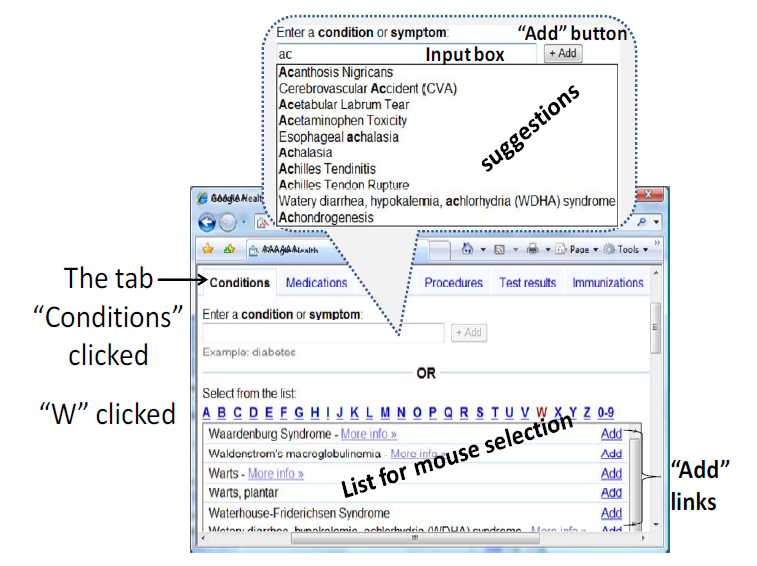
\includegraphics[width=0.7\textwidth]{fig/WebSideChannelExample1.png}
		\caption{Example Health Record System from \cite{WebSideChannel}}
		\label{Fig: HealthRecordSystem}
	\end{figure}
	
	In this example, the authors demonstrated that according to which tab or alphabet the user has clicked, the server returns a series of  packets with distinguishable lengths and directions. Further more, distinguishable packet traces can also be observed when user types in the input box triggering auto suggestion. As a result, an eavesdropper can deduce the user input simply by looking at the packet features of encrypted traffic.
\end{example}

\begin{example}
	The second vulnerable website is an online taxing service. In this system, the tax application form varies due to the payee's family status. The vulnerability of this website is that users are directed to different pages according to the form they are going to fill, while different pages results into packets of different lengths and directions, allowing an eavesdropper to reveal the family status of the user. The packet features of encrypted traffic again breached the data confidentiality.
\end{example}

%Financial Graph Example

%Search Keyword Example (briefly, refers to the other one)

\subsection{Traffic Analysis Countermeasures}




\section{Methodologies in Information Leakage }


\chapter{Experiment Setup} \label{Chp: Experiment Setup}
%All experiments are done within the Cooja simulator. The environment we simulated is as described in \Cref{fig: Setup}.

In this chapter we describe how we set up our experiments. The related source code can be downloaded from: \url{https://github.com/Salties/MyRepository} .

\section{Overview}

\Cref{Fig: Experiment Setup} illustrates an overview of our experiment setup. 

\begin{figure*}[h!]
	\center
	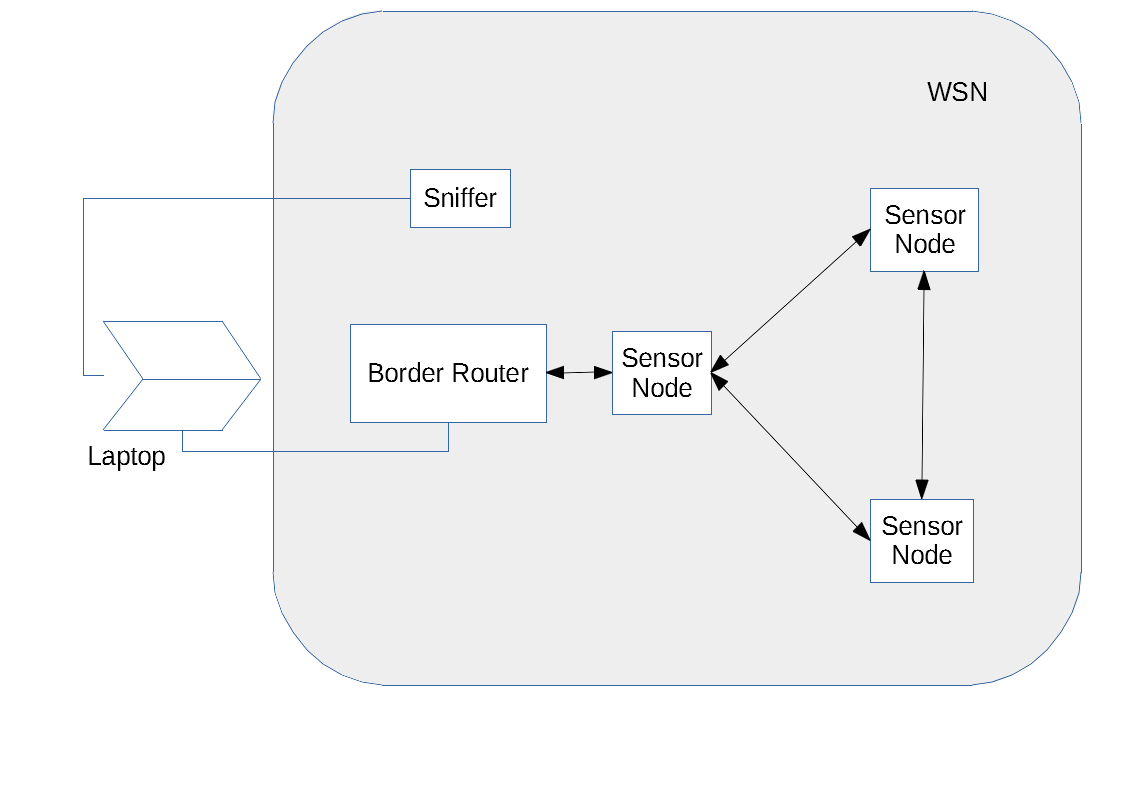
\includegraphics[width=0.75\textwidth,]{fig/setup.png}
	\caption{Experiment Setup} \label{Fig: Experiment Setup}
\end{figure*}

\begin{description}[style=nextline]
	\item[WSN]
	The greyed area on the right inside the rectangle of \Cref{Fig: Experiment Setup} represents a 6LoWPAN network as described in \Cref{Chp: Building Blocks}. The topology is dynamic as explained in \Cref{Sec: Network Layer}.  We make no further assumptions about the application for generality in this report.
	
	\item[Sensor Node]
	Each Sensor Node is a WSN device that supports the protocol suite described in \Cref{Tbl: Summary of WSN Building Blocks}. All Sensor Nodes are connected to the same 6LoWPAN network. We do not impose the use of CoAP in our setup; instead, we consider applications may directly invoke UDP (or DTLS) interfaces. 
	
	\item[Border Router]
	Border Router is a special instance of Sensor Node. Comparing to normal Sensor Nodes, Border Routers are specifically used to bridge other devices to the Sensor Network. In our experiments, Border Routers are connected to Laptops through USB connections. From a perspective of other Sensor Nodes in the WSN, a Border Router appears no different to the others. In many real world applications, the Border Router is connected to a management machine and serves as the DODAG root, but this is not necessarily the case in our experiments.
	
	\item[Sniffer]
	Sniffer is another special instance of Sensor Node. The Sniffer passively captures all frames it receives and does not transmit anything at all; thus it is transparent to other Sensor Nodes in the network. In our setup as of \Cref{Fig: Experiment Setup}, the Sniffer pipes any frames it captured to the Laptop. From a practical aspect, the hardware device of a Sniffer has a limited effective radius and thus would not be able to capture all frames in wide range WSNs; however this can be easily overcame by deploying multiple Sniffers to cover a wider area. In our experiments, we simply assume every frame in the WSN is visible to the Sniffer.
	
	\item[Laptop]
	The Laptops in our experiments usually represent adversaries with unequally supreme resources comparing to the Sensor Nodes in terms of energy, memory and computational power. In our setup of \Cref{Fig: Experiment Setup}, the Laptop, which represents an adversary, has access to all traffic captured by the Sniffer and is allowed to interact with other Sensor Nodes if the Border Router is compromised through external methods.
\end{description}

\section{Operating System}

We use Contiki\cite{Contiki} to build our experiments.  Our source codes are tested with Contiki release-3.0 which is available at: \url{https://github.com/contiki-os/contiki/releases/tag/3.0} .

\subsection{Brief Introduction to Contiki:}

The official instruction for using Contiki is available at:	\url{http://www.contiki-os.org/start.html} .


Contiki is an open source embedded system crafted for IoT devices. It has a good support on many recent hardware and it is optimised for code size. Contiki does not provide any direct User Interfaces, UI, by default. Instead, the embedded system provides a framework for developers to use C language to write (mostly) hardware portable codes, as well as providing a set of APIs including clock library, simple process management and network interfaces, etc.

To use Contiki, there are basically three steps:

\begin{enumerate}
	\item Write the application code in C. There are plenty examples in Contiki source code those can be used as frameworks.
	\item Compile the source code according to the target device through \textit{make} command. Note that the root of Contiki source code must be correctly specified in the \textit{makefile}. 
	\item Upload (also called ``burn'') the binary code to your device. 
\end{enumerate}

The application code is automatically executed whenever the device is powered on.

\section{Devices}

Three platforms are adopted in our experiments:

\begin{itemize}
	\item \textbf{TelosB}\cite{TelosB}, also known as Sky mote. This is a popular device for WSNs featuring low cost. As a trade off, TelosB has only very constrained performance in terms of bandwidth, available code size and processing power.
	
	\item \textbf{CC2538}\cite{CC2538}. This is a relatively powerful platform with an ARM-Cortex M3 processor. To our knowledge, this is one of the becoming dominant device used in WSN applications.
	
	\item \textbf{Wismote}\cite{Wismote}. This platform can be considered as a performance upgraded version of TelosB. Note that we only use Wismote in simulator. When using our code, one needs to modify the Contiki compiling system follow the instructions in: \url{https://github.com/contiki-os/contiki/wiki/MSP430X} .
\end{itemize}

All these nodes are 802.15.4\cite{802154} compatible and does not have any sensor attached by default. We omit further hardware details as it is beyond the scope of this project. 

\subsection{Cooja Simulator}

The Contiki source code includes the Cooja simulator under its tools folder. The official instruction for using the Cooja simulator is available at: \url{http://www.contiki-os.org/start.html} .

Cooja provides simulation for a whole WSN application. It generates simulated data for serial output, LED status and radio traffic, etc. An example of Cooja simulation is shown in \Cref{Fig: An Example of Cooja Execution}.

\begin{figure*}[h!]
	\center
	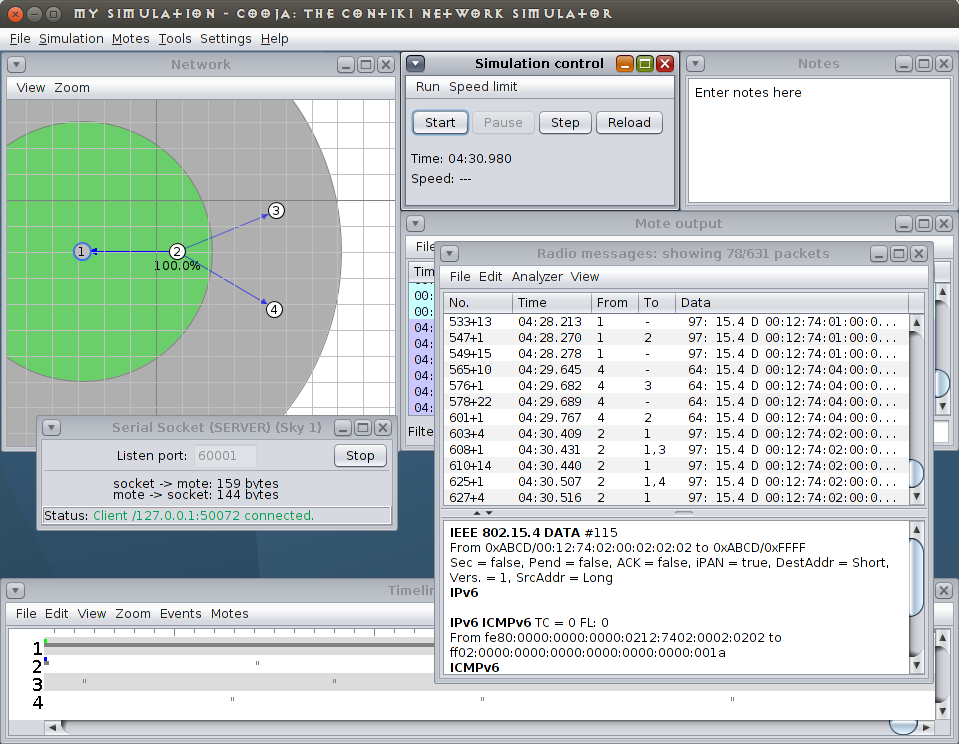
\includegraphics[width=0.8\textwidth]{fig/cooja_example.png}
	\caption{An Example of Cooja Execution}
	\label{Fig: An Example of Cooja Execution}
\end{figure*}

\Cref{Fig: An Example of Cooja Execution} shows a simulation simulating the exact same WSN topology as described in \Cref{Fig: Experiment Setup}, with \textcircled{1} being the Border Router. 

In this project, we are mostly interested in the radio traffic. The traffic is captured by the ``Radio messages'' plugin which exactly serves as the Sniffer in \Cref{Fig: Experiment Setup}. The corresponding pcap file is written by Cooja alongside the simulation under ``cooja/build/'' folder, which can later be opened by Wireshark\cite{Wireshark} for analysis, as shown in \Cref{Fig: A Wireshark Example}.

\begin{figure*}[h!]
	\center
	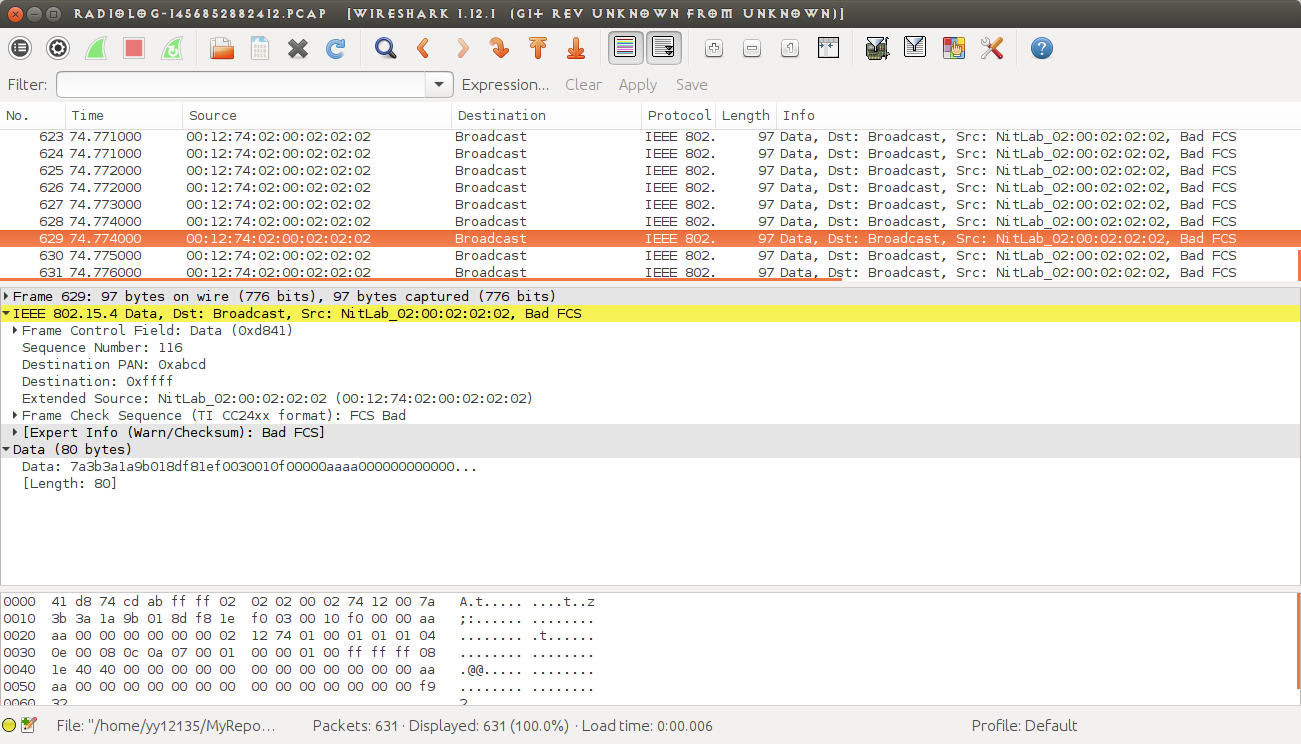
\includegraphics[width=0.8\textwidth]{fig/wireshark_example.png}
	\caption{A Wireshark Example}
	\label{Fig: A Wireshark Example}
\end{figure*}

As of the time of writing this report, Cooja in Contiki release-3.0 supports simulations for TelosB and Wismote. CC2538 is not yet supported in the latest version.

Cooja is not suitable for large scale experiments as there is a potential memory leakage problem which drastically downgrades long time simulations, or sometimes even crashes them. Also notice that the performance of Cooja is obviously better on low performance devices. For example, simulations with TelosB are nearly 8 times efficient than Wismote for the same application code.

\section{Security Measures}

In this report, we analyse traffic that is protected by two security measures implemented on Contiki release-3.0, namely noncoresec and DTLS.

\subsection{noncoresec}

In Contiki source code, LLSEC is an alias for \textit{noncoresec}.

\textit{noncoresec}\cite{noncoresec}\cite{LLSEC} is a reduced 802.15.4 Security implementation on Contiki. \textit{noncoresec} uses a hard coded network shared key that is defined by the ``NONCORESEC\_CONF\_KEY'' macro in ``project-conf.h'' file; thus it cannot be updated during runtime. 

When \textit{noncoresec} is enabled, we always assume it uses the highest Security Level (7), i.e. all frames are encrypted and authenticated in AES-128-CCM* mode with 16 bytes MAC, as described in \Cref{Subsec: 802154 Sec}. With this Security Level, all Sensor Nodes in the WSN must have the same key that is hard coded during compilation. External Sensor Nodes without the key cannot send or receive any frame and thus are repelled from the network.

In scenarios where the WSN is protected by \textit{noncoresec}, we always assume the adversary has no knowledge of the key. This effectively indicates that the adversary is unable to join the network at all since he cannot receive or send any frames as we explained above.

Our code using \textit{noncoresec} are successfully tested on all our devices. However, even though CC2538 has an AES coprocessor built in, the current version of Contiki code does not utilise this feature at all; instead, it uses a textbook software AES implementation as on other platforms. Also notice that the source code of \textit{noncoresec} is only included for TelosB platform by default. When using on other platforms, the developer needs to manually add its source code into the platform specific building system.

\subsection{DTLS} \label{Subsec: Experiment DTLS}

DTLS in Contiki is supported by a third party module \textit{tinydtls}\cite{tinydtls}. \textit{tinydtls} is originally developed for desktop systems and is later ported to Contiki. In the current version tinydtls-0.8.2, there are two cipher suites supported:

\begin{enumerate}
	\item TLS\_ECDHE\_ECDSA\_WITH\_AES\_128\_CCM\_8\cite{rfc7251}
	\item TLS\_PSK\_WITH\_AES\_128\_CCM\_8\cite{rfc6655}
\end{enumerate}

The use of cipher suite can be configured at compiling time by using the ``configure'' script under ``tinydtls-0.8.2'' folder. Also notice that when used with Contiki, ``--with-contiki'' argument is also required when running this script. By default, TLS\_ECDHE\_ECDSA\_WITH\_AES\_128\_CCM\_8 is preferred by the tinydtls implementation.

The keys (or master secrets) can be configured at runtime by using an interface provided by the tinydtls module. When using TLS\_PSK\_WITH\_AES\_128\_CCM\_8, where PSK stands for Pre Shared Key, the same master secrets must be coded beforehand into the clients and servers, or derived by external key management schemes.

The code from the tinydtls official website cannot be directly used on our platforms. The ``tinydtls-0.8.2'' folder in our source code contains a version of code we have tuned for our platforms. When using our code, the following problems should be noticed:

\begin{enumerate}
	\item TelosB does not support tinydtls as the code is oversized and cannot fit into the ROM of this device. Also notice that it cannot transmit frames longer than 127 bytes neither; thus any DTLS handshake message need avoid this type of Sensor Nodes in its path, as packets exceeding this length will be silently dropped by these nodes.
	\item Wismote with TLS\_ECDHE\_ECDSA\_WITH\_AES\_128\_CCM\_8 causes a crash of simulator. We have not yet figure out the exact cause of this problem. A potential cause might be illegal memory access in arithmetic operations.
	\item MTU specified by 802.15.4 Standard is 127 bytes whilst several DTLS handshake messages exceed this limitation. This constriction can be loosen by specifying\\ UIP\_CONF\_BUFFER\_SIZE, QUEUEBUF\_CONF\_NUM and UIP\_CONF\_RECEIVE\_WINDOW macros in ``project-conf.h'' file to a larger value. Nevertheless, specifying larger MTU does not guarantee the success transmission of packets. The handshake packets exceeding 127 bytes would still potentially be silently dropped during runtime.
	\item The handshake packets retransmission should be avoided at best effort. The restransmission implementation of tinydtls should not be relied on as sometimes it is not triggered by a packet lost, potentially due to a signal loss in the Contiki kernel. When a packet is lost during the handshake, the client and server will potentially freeze, resulting into a deadlock. Our current solution is to simply restart the procedure from the beginning, or simply reboot the devices.
	\item TLS\_ECDHE\_ECDSA\_WITH\_AES\_128\_CCM\_8 has a performance issue. Even on CC2538, each curve computation costs roughly 80 seconds on each side. This performance issue somehow triggers other problems in a chain reaction resulting into malfunctioning of the application code. The first problem is that the computation time exceeds the DTLS timeout, which therefore triggers the retransmission problem we described above. We have solved this problem in our code by increasing the timeout. The second problem happens when using  unequal computational power on client and server side, e.g. trying to perform a DTLS handshake from the Laptop through Border Router as the client to a CC2538 Sensor Node in the network. The unequal computational power leads to the fact that the Laptop processes the handshake packets immediately and continuously sends out the responses, without waiting for the Sensor Node to complete its computation. Consequently, the buffer of Sensor Node is instantly over flooded by the handshake packets resulting into some of them being dropped, which, again, triggers the problems caused by retransmission we described above. Our solution to this problem is to simply add a \textit{getchar()} into DTLS client of the Laptop side, of which asks a key stroke before sending each packet
%	\item Multi sessions is not well supported in the current tinydtls implementation on Contiki due to some memory management problem. In another word, try not to establish multiple DTLS sessions with one DTLS server running on the same Sensor Node. Further more, there is a potential memory leakage in tinydtls on termination of a DTLS session, which therefore could potentially crash the application or simulation. 
\item tinydtls is designed with asynchronous I/O. One must carefully designs the application code to use it.
\end{enumerate}

In experiments with DTLS, we consider the adversary is a group of compromised Sensor Nodes in the WSN. In other words, not only having all access to packet transmitted over the network, the adversary is capable to send any crafted packets to any Sensor Node in the network as well. In experiments with TLS\_PSK\_WITH\_AES\_128\_CCM\_8 being the cipher suite, we assume the adversary has no knowledge of the pre shared keys in any other paired Sensor Nodes; otherwise any ciphertext is immediately broken. Similarly, when TLS\_ECDHE\_ECDSA\_WITH\_AES\_128\_CCM\_8 is used, we assume the adversary has no knowledge of the private keys in other Sensor Nodes. In reality, such compromised Sensor Nodes can be Border Routers connected to adversary controlled Laptops deployed among the WSN. .

\subsection{Overloading noncoresec and DTLS}

Theoretically, it is possible to overload noncoresec with DTLS since they are implemented at different layers in the protocol stack. In another word, one can technically use noncoresec to provide MAC Layer security while using DTLS to provide Application Layer security.

However, in Contiki we noticed that either of them de facto adopts AES-128 with CCM mode as the underlining encryption method. Cryptographically speaking, the encryption part of AES-128 with CCM can be viewed as a pseudo random bit stream generator and overloading both of them is equivalent to use another pseudo random bit stream that is the XOR of them. To our knowledge, it is unclear whether this provides more randomness or not. However, intuitively under the assumption that AES-128 can be viewed as a pseudo random function, we argue that this overload does not seem to provide any more confidentiality. The same applies to the CBC-MAC.

On the other hand, the performance impact of overloading cannot be ignored in WSNs. In fact noncoresec and DTLS adds 23 bytes and 21 bytes overhead to each packet respectively whereas the MTU specified by 802.15.4 Standard is only 127 bytes, overloading them will immediately adds great overhead in terms of bandwidth and thus energy consumption. 

Hence, we argue that overloading is not practical and thus is excluded from our experiments.

\section{Applications} \label{Sec: Applications}

In this section we explain some simple applications we have developed in our experiments. These applications are aimed to cover the most generic scenarios of WSN applications. The source code of the applications are located in the ``experiments'' folder in our source code. 

\begin{description}[style=nextline]

	\item[{dtls-telnet}]
	This tool is a DTLS client runs on Linux. It establishes a DTLS session with a DTLS server and runs a telnet application that reads and sends data in ASCII. We use this tool in most of our experiment as the DTLS client. It is located under the ``tools'' folder in our source code.
	
	\item[{dtlsbr}]
	{dtlsbr} is a DTLS echo server merged with a Border Router application running concurrently. An echo server echoes everything received from the clients similar to PING. {dtlsbr} is developed to study how the tinydtls implementation affects the packet features.
	
	\item[{borderest}]
	{boderest} is a CoAP server merged with a Border Router application running concurrently. This application is used to predict some traffic features with CoAPs. Even though there is no security measure adopted in this application, we expect that most of the packet features should be linearly preserved with CoAPs as we explained in \Cref{Subsec: CoAPs}. This application is not compatible with TelosB due to code oversize.
	
	\item[{keydtls}]
	{keydtls} is developed to study how different DTLS session keys affect the packet features. The Sensor Node runs a DTLS server and reads client input, responses with a random string in ASCII representing a sensor reading.
	
	\item[{keyllsec}]
	{keyllsec} is developed to study how different noncoresec keys affect the packet features. There are two sub-applications in this application:
	\begin{itemize}
		\item \textbf{broadcast} application broadcasts an arbitrary message periodically.
		\item \textbf{unicast-sender} and \textbf{unicast-receiver} are a pair of applications where the sender periodically pushes an arbitrary message to the receiver.
	\end{itemize}
	These applications are protected by noncoresec.

	\item[{dtlseiri}]
	\textit{dtlseiri} is developed to study how the execution time of code on a DTLS server affects the time interval of response. Similar to {keydtls}, {dtlseiri} repeatedly calls the Contiki random number generator to generate a random ASCII string as response, representing a sensor reading with additional processing. The execution time is controlled by the number of calls to the random number generator. 

%application detection dtls PINGLOAD
	\item[{dtlspingload}]
	This application is identical to \textit{dtlseiri} but developed for a different purpose. It is used to study a potential side channel attack we named ``pingload'' which we explain in later chapters.
\end{description}

\section{Summary}

In this chapter, we described how our experiments are set up. Two security measures are used in our experiments, namely noncoresec and DTLS. 

We summarise the compatibility of the security measures to the platforms in our experiments as \Cref{Fig: Compatibility of Platforms and Security Measures}.

\begin{table}[h!]
	\center
	\begin{tabular}{|c|c|c|c|}
	\hline
	\multirow{2}{*}{} & \multirow{2}{*}{noncoresec} & \multicolumn{2}{c|}{DTLS} \\ \cline{3-4} 
	                  &                             & ECDHE\_ECDSA & PSK        \\ \hline
	TelosB            & \checkmark                  & N/A          & N/A        \\ \hline
	CC2538            & \checkmark                  & \checkmark   & \checkmark \\ \hline
	Wismote           & \checkmark                  & N/A          & \checkmark \\ \hline
	\end{tabular}
	\caption{Compatibility of Platforms and Security Measures}
	\label{Fig: Compatibility of Platforms and Security Measures}
\end{table}

We have also developed several simple applications to model the most typical WSN application scenarios. We summarize their compatibility in \Cref{Fig: Compatibility of Platforms and Applications}.

\begin{table}[h!]
	\center
	\begin{tabular}{|c|c|c|c|c|c|c|}
	\hline
	\multirow{2}{*}{} & noncoresec & \multicolumn{4}{c|}{DTLS}                           & No Security \\ \cline{2-7} 
	                  & keyllsec   & dtlsbr     & keydtls    & dtlseiri   & dtlspingload & boderest    \\ \hline
	TelosB            & \checkmark & N/A        & N/A        & N/A        & N/A          & N/A         \\ \hline
	CC2538            & \checkmark & \checkmark & \checkmark & \checkmark & \checkmark   & \checkmark  \\ \hline
	Wismote           & \checkmark & \checkmark (*) & \checkmark (*) & \checkmark (*) & \checkmark (*)   & \checkmark  \\ \hline
	\end{tabular}
	\caption{Compatibility of Platforms and Applications}
	\label{Fig: Compatibility of Platforms and Applications}
	(*): As explained in \Cref{Subsec: Experiment DTLS}, on Wismote DTLS can only be used with\\ TLS\_PSK\_AES\_128\_WITH\_CCM\_8.
\end{table}



%A table for available combinations

%\begin{itemize}
%\item{\bf Adversary} is a malicious party that tries to illegally reveal information from the encrypted traffic.
%\item{\bf Border Router}, or BR, is a device that connects adversary to the sensor network. \textbf{BR is not allowed when LLSEC is enabled} as the adversary does not have the key and hence cannot connect into the network. We will discuss more about LLSEC in \Cref{Chp: LLSEC}.
%\item{\bf Sniffer} passively captures all traffic in the network. 
%\item{\bf Target} and {\bf Nodes} are sensors deployed in the sensor network. They communicates to each other through encrypted channels.
%\item{\bf Sensor Network} discussed in this paper is a 6LowPAN network based on Contiki OS.
%\end{itemize}

%Realistically speaking, this scenario could happen say an adversary sitting near a smart house with a laptop attached to a SoC\footnote{System on Chip} device, or your malicious neighbour walks into your smart house with her smart phone.
%
%\section{Adversary Power}
%The powers assumed in the experiments are considered to be practical in real life.
%
%When LLSEC is enabled, all traffic, including RPL\footnote{Routing Procol for Low-power and Lossy Networks} messages, are encrypted; therefore no external nodes can connect to the network as an external node cannot send any valid RPL messages to join the network. The adversary only passively sniffs all traffic.
%
%With LLSEC disabled, the adversary can therefore join the sensor network through a BR and hence is also capable to send messages to the target(s). However, she will not be able to inject any message into an encrypted channel such as a DTLS channel.
%
%\section{Types of Packets}
%We simply categorise the packets into two types:
%\begin{itemize}
%\item {\bf Network Management Packets}: These are the packets generated by the protocols to  maintain the functionality of network, such as MAC ACKs, RPL messages or ICMP messages.
%\item {\bf Data Packets}: These are those packets generated by applications running on sensor nodes., such as a CoAP packet.
%\end{itemize}
%
%This is only a subjective rough categorisation and may not be precise. For example an TCP data packet may set its ACK flag, or DTLS handshake packets could ambiguously fall into both categories. However, we ignore this ambiguity as it is not our focus.
\chapter{Link Layer Security}

\section{Non core security}

\section{802.15.4 security}

\section{Reset Problem}

\section{Distinctive packet length for RPL packets}

\chapter{DTLS}
DTLS has potentially the best interoperability as it is an variation of the widely used TLS in Internet. However, its design might not fit into the nature of WSN for practical reasons.

\section{Implementation Issues}
tinydtls\cite{tinydtls} currently supports two ciphersuites, namely TLS\_PSK\_WITH\_AES\_128\_CCM\_8 and TLS\_ECDHE\_ECDSA\_WITH\_AES\_128\_CCM\_8. 

However, we encountered several difficulties when trying to set up a  network with DTLS.

\begin{description}
\item[Low Computational Power] \hfill \\
Curve computation requires relatively a large amount of computational power. Even using a relatively power platform (CC2538), it still takes minutes to complete a DTLS handshake with
TLS\_ECDHE\_ECDSA\_WITH\_AES\_128\_CCM\_8.

\item[Low Bandwidth] \hfill \\
The 6LowPAN standard specifies that the minimum MTU is 127 bytes whilst 67 (87 with LLSEC) bytes are occupied by protocol headers until UDP, which leaves 60 (40 with LLSEC) bytes available for UDP layer payload. This value can be easily exceeded even during the handshake, such like using a longer key. Some attempts have been made to solve this issue, e.g. CoDTLS\cite{CoDTLS}\footnote{This draft has been abandoned for some reason we do not know.}.

\item[Code Size] \hfill \\
The tinydtls fails to fit into some devices, e.g. skymote, as its size of code is too large.
\end{description}

Therefore although TLS\_PSK\_WITH\_AES\_128\_CCM\_8 is less flexible (and probably less secure) as it uses a pre-shared master secret than TLS\_ECDHE\_ECDSA\_WITH\_AES\_128\_CCM\_8, it is still considered to be a relatively practical security measure as it requires less resources.

\section{No multicast support}
Some application protocols, such as CoAP, utilises the multicast feature of 6LowPAN whilst TLS is a protocol designated for securing communications between two parties, so is DTLS.

\section{Overloading DTLS with LLSEC}
Adopting both security measures at the same time is possible as they are implemented at different layers. However, it is questionable whether this will bring more security, as both {\it noncoresec} and TLS\_PSK\_WITH\_AES\_128\_CCM\_8 are using 128 bit AES with CCM mode as their cryptographic primitive.

\chapter{Application Detection}
Similar to website fingerprinting, we try to identify the application running on target note by its traffic. This chapter discusses some general idea without a specific application.

\section{Network Protocol Headers}
Since most information in MAC\footnote{Media Access Control, not to be confused with the cryptographic term Message Authenticate Code.}, IP and UDP headers are related to routing and network maintenance and thus independent except the length fields and CRC\footnote{Cyclic Redundancy Check, a code to detect or correct transmission error}. 

\section{Packet Length}
Packet length is usually the most interested target in traffic analysis. However, packet lengths are also highly application dependant; thus we are not pursuing this topic further without a specific application.

\section{Timing Packet Response}
Unlike web applications where the client and server are usually physically distant, sensor networks can sometimes located in a concentrated area, such as a house which its radius can be less than 10 meters. 

These features theoretically enables one to capture all traffics in such a sensor network. As opposed to the case of Internet where packets are usually timed on the client’s side and thus network latency (RTT\footnote{Round-Trip Time}) must be concerned, being able to capture all traffic in the network provides  much more accurate timing information and hence may be exploited to develop more efficient attacks.

\begin{definition}
In a Request-Response application model, \textbf{RI}, {\bf Response Interval}, is defined as the interval between a request packet being received and its response being sent.
\end{definition}

\begin{example}
\begin{figure}
\centering
{
	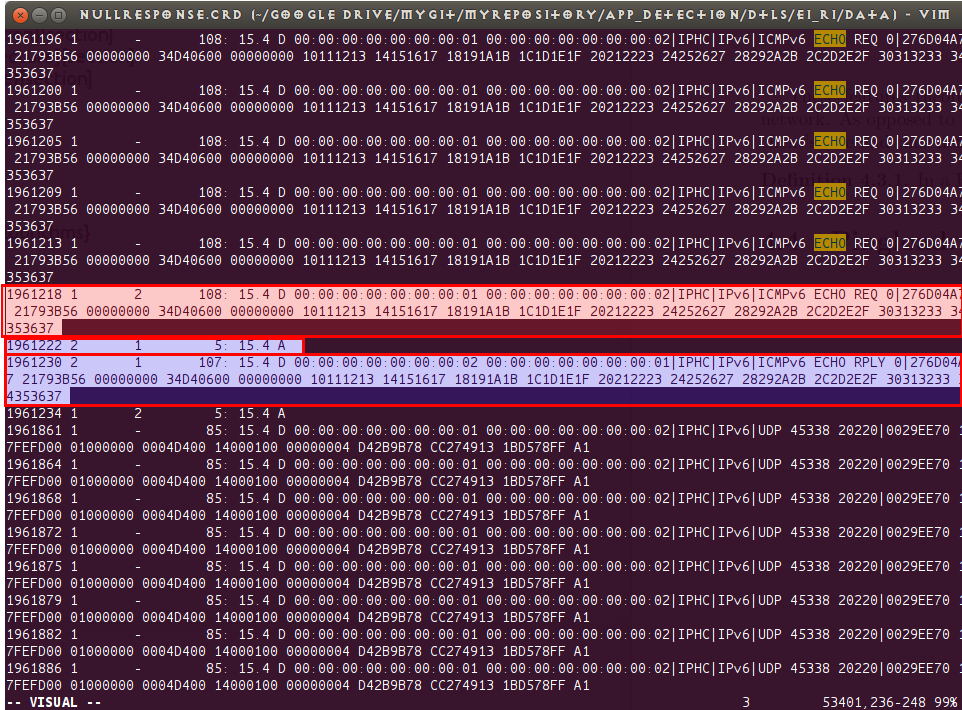
\includegraphics[width=\textwidth,]{fig/responsetime.png}
}
\caption{Capture of a ping packet}
\label{fig: ping packet}
\end{figure}

\begin{table}[!]
\centering
\begin{tabular}{|l|l|l|l|l|}
\hline
Time (ms) & From (ID) & To (ID) & Length (bytes) & Type          \\ \hline
1961218   & 1         & 2       & 108            & ICMP ECHO \\ \hline
1961222   & 2         & 1       & 5              & 802.15.4 ACK  \\ \hline
1961230   & 2         & 1       & 107            & ICMP ECHO \\ \hline
\end{tabular}
\caption{Packet Features of an ICMP ECHO request and response}
\label{Tbl: ping}
\end{table}

Three packets are marked out in \Cref{fig: ping packet} which forms an instance of ICMP ECHO\cite{rfc1122} (also known as PING) session. The extracted packet features are displayed in \Cref{Tbl: ping}.

\begin{description}
\item[Explanation of the Packets:]\hfill \\
The first packet is an ICMP ECHO request and the third packet being its response. The second packet is a 802.15.4 ACK\footnote{This is an acknowledgement from the receiver that notifies the sender that the packet has been received.} and is thus transparent to the upper ICMP protocol.
\end{description}

From this example we can see that the RI for this PING session is:
\begin{equation*}
1961230 - 1961218 = 12 \text{(ms)}
\end{equation*}

\end{example}

Timing information can be exploited by several attacks, such as \cite{Peekaboo} and \cite{rsatiming}.

We have experimentally measured a RNG\footnote{Random Number Generator} call on Wismote platform in the Cooja simulator is roughly 0.3 ms.

\section{PINGLOAD: PING side-channel for Payload }
Support of ICMP ECHO is required by \cite{rfc1122} and is also enabled in Contiki OS by default. However, our experimental results shows that the response time of these ping packets could potentially be exploited to reveal the application running on target sensor node.

We call such technique {\bf  Application Fingerprinting}.

\subsection{Hypothesis}
A phenomenon we realised is that when a ping packet arrived while the target node is executing some payload, say reading a sensor or processing data, the PING RI begins to vary comparing to a stable value  when no there is no payload. 

\begin{example}
\begin{figure}
\centering
{
  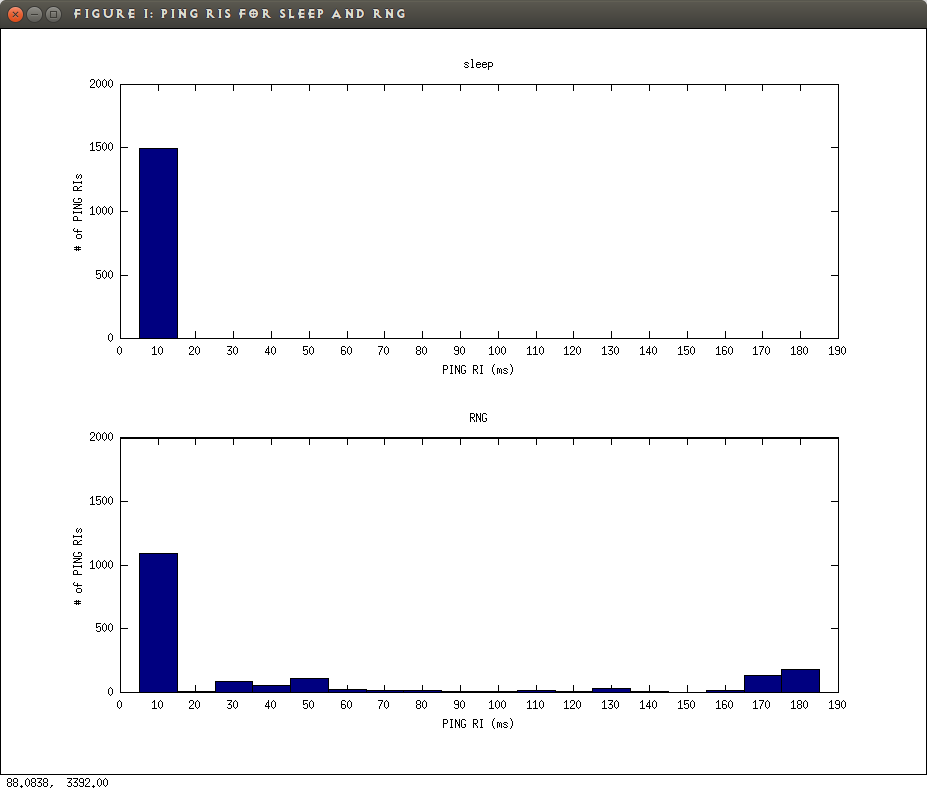
\includegraphics[width=1\textwidth]{fig/pingri.png}
}
\caption{An example of PING RIs with different payload}
\label{Fig: PINGLOAD RIs}
\end{figure}
\Cref{Fig: PINGLOAD RIs} shows RIs of PING collected in two experiments. The upper half are collected with the target is constantly sleep whilst the lower half occasionally receives a request which triggers the target to call RNG. We can see that the PING RI varies alongside the target is given some payload from this figure.
\end{example}

The data shown in \Cref{Fig: PINGLOAD RIs} suggests that the “plain”, that is without any interference, PING RI is 12 to 13 ms. Further more, those variations of  PING RI is very likely caused by the payload of the target.

This experiment inspired that the distributions of PING RIs might vary according to the payload of target and could possibly considered as an fingerprint of the target’s application. In other word, an adversary could possibly tell whether the target is running a specific application by looking at its PING RIs distribution.

The attack is strait forward:
\begin{description}
\item[Profile sleep RIs]: \hfill\\
The PING RIs for a sleeping node of the same platform can be profiled by pinging a sleeping node. We denote the sleeping profile as $RI_{sleep}$. 

\item[Fingerprint application]: \hfill\\
The adversary collects PING RIs on a profiling node with known application. The profiling node needs to be of the same platform and executing the same code of the target’s. The application fingerprint denotes as: $F_p=\{p_1, p_2, ... , p_n\}$. 

\item[Collect fingerprint of target]: \hfill\\
The adversary then collects the PING RI for the target node by pinging it. We denote the collected data as: $F_t=\{t_1, t_2, ..., t_m\}$.

\item[Extract Featured RIs]: We can remove them from the data sets and keep the PING RIs those has been interfered by the application. We denote the extracted RIs as \textbf{Featured RIs}:
\begin{eqnarray*}
F’_p = \{x | x \in F_p,  x \notin RI_{sleep}\}\\
F’_p = \{x | x \in F_t,  x \notin RI_{sleep}\}
\end{eqnarray*}

Practically speaking, the PING protocol are designed to be responded immediately for diagnosis purpose; hence $RI_{sleep}$ usually has an extremely low variance and its mean is also much less than $F_p$ and $F_t$.

Using the Featured RIs not only provides a better vision of the fingerprint but also removes the error caused by different frequency of the target code being executed, as all the Featured RIs are actually collected when the node is at a non-sleeping state. 

\item[Estimate Distribution (Optional)]: \hfill\\
We then estimate the distributions of $F’_p$ and $F’_t$, denote as $D_p$ and $D_t$. A naive method is to simply use their histograms. An example of such histograms are shown as \Cref{Fig: featuredri_rng}.

\begin{figure}
\center
{
	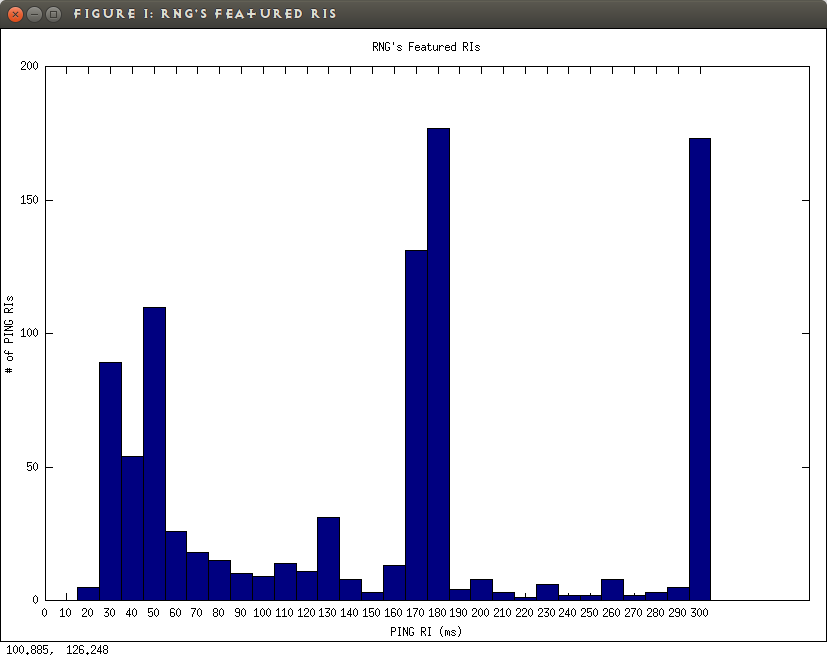
\includegraphics[width=0.49 \textwidth]{fig/featuredri_rng1.png}
	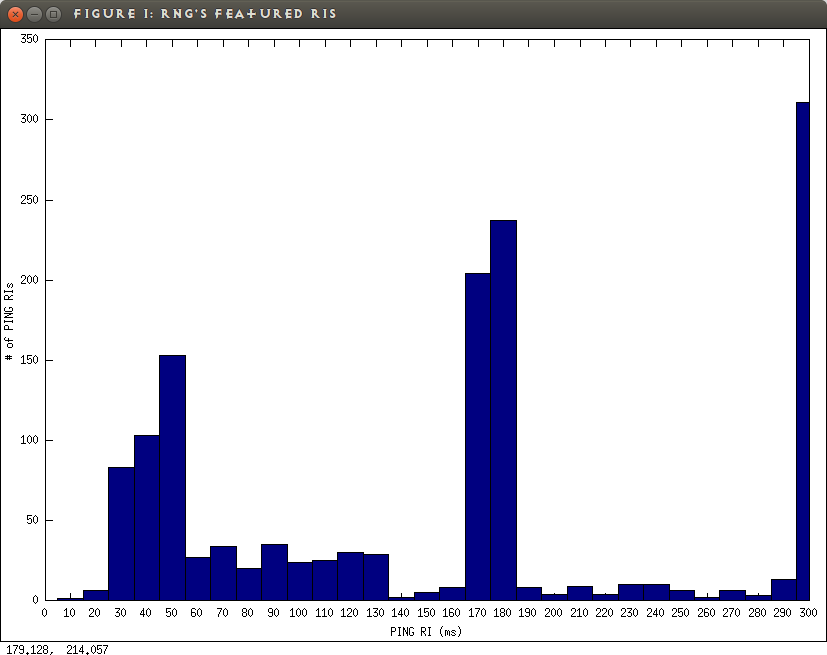
\includegraphics[width=0.49 \textwidth]{fig/featuredri_rng2.png}
}
\caption{Two examples of RNG’s Featured RIs histogram}
\label{Fig: featuredri_rng}
\end{figure}

\item[Distinguish Distributions]: \hfill\\
Finally we test whether $D_t$ and $D_p$ are the same distribution. An naive way is to compute the correlation of counts of the histograms. We conclude the target node is running the profiled application if $D_t$ and $D_p$ are the same distribution.
\end{description}

Practically speaking, the key point of Application Fingerprinting is to test whether the target’s Featured RIs, i.e. $F’_t$, is sampled from same distribution of the profiled one, i.e. $F’_p$; therefore estimating their distribution might not be necessary for some statistical methods such as t-tests. However as we can see in \Cref{Fig: featuredri_rng}, PING RIs’ distribution are very unlikely to be normalised. Therefore a future work is to find a better distinguishing method than the current naive one.

\subsection{Experiment Result}
We tried our Application Fingerprinting method above on a Cooja simulated Wismote platform with different code. \textbf{In conclusion, the fingerprint appears to be effective for certain circumstances but will tends to result into false positives as the profiled application and target application gets similar to each other.}

To be more specifically, the target node execute some specific code upon receiving an application layer protocol request, similar to CoAP. Further more, all traffic are protected by DTLS with TLS\_PSK\_WITH\_AES\_128\_CCM\_8 ciphersuite. Both intervals of PINGs and the application request are set to some asynchronised value to avoid overflooding the target and to create a ‘more realistic’ simulation.

Everything other than the examined code are the same for all experiments. Two samples are collected independently for each code to simulate a fingerprinting scenario. The histograms are clustered by 5ms.

We examined two classes of codes:
\begin{description}
\item[RNG Calls]: \hfill\\
The target node repeatedly calls RNG for $i$ times. We examined their Featured PING RI for different values of $i$. The reason for picking RNG is that on some platforms where a hardware RNG is provided, the call to it is expected to be similar to a call to a sensor reading which is actually an interrupt. Results are shown in \Cref{Tbl: pingload RNG}.

\item[Arithmetic Operations]: \hfill\\
The target node repeatedly does arithmetic operations, namely addition, multiplication and modular, on two random generated word size integers for 10000 times. This class is particularly interested from a cryptographic point of view as the number of arithmetic operations could potentially developed to key recovering attacks. Results are shown in \Cref{Tbl: pingload arth}.
\end{description}



\begin{table}
\centering
\begin{tabular}{|c|cccc}
\hline
\textit{\textbf{Correlations}} & \multicolumn{1}{c|}{i=50} & \multicolumn{1}{c|}{i=100} & \multicolumn{1}{c|}{i=2500} & \multicolumn{1}{c|}{i=5000} \\ \hline
i=50                           & \textbf{0.988}            & 0.891                      & -0.014                      & -0.033                      \\ \cline{1-1}
i=100                          & 0.891                     & \textbf{0.973}             & -0.025                      & -0.042                      \\ \cline{1-1}
i=2500                         & -0.014                    & -0.025                     & \textbf{0.993}              & -0.035                      \\ \cline{1-1}
i=5000                         & -0.033                    & -0.042                     & -0.035                      & \textbf{0.985}              \\ \cline{1-1}
\end{tabular}
\caption{Correlations for RNG}
\label{Tbl: pingload RNG}
\end{table}

\begin{table}
\centering
\begin{tabular}{|c|ccc}
\hline
\textit{\textbf{Correlations}} & \multicolumn{1}{c|}{+} & \multicolumn{1}{c|}{*} & \multicolumn{1}{c|}{\%} \\ \hline
+                              & \textbf{0.990}         & \textbf{0.990}         & \textbf{0.988}          \\ \cline{1-1}
*                              & \textbf{0.990}         & \textbf{0.989}         & \textbf{0.985}          \\ \cline{1-1}
\%                             & \textbf{0.988}         & \textbf{0.985}         & \textbf{0.984}          \\ \cline{1-1}
\end{tabular}
\caption{Correlations for word arithmetic operations}
\label{Tbl: pingload arth}
\end{table}

\begin{table}[]
\centering
\begin{tabular}{|c|c|}
\hline
\textbf{\textit {Correlations}} & +     \\ \hline
i=50         & 0.877 \\ \hline
\end{tabular}
\caption{Correlation for $i=50$ and addition}
\label{Tbl: pingload rng arth}
\end{table}

We also computed the correlation for $i=50$ and addition, as shown in \Cref{Tbl: pingload rng arth}.

The results suggests the following conjectures:
\begin{enumerate}
\item The results for RNG suggests that the fingerprinting is effective for this class of code, as the same code results into nearly perfect correlations ($\geq 0.95$).

\item Even relatively slight changes can be detected, as we can see the correlation dropped to $0.891$ alongside 50 iterations of RNG calls (50 RNG calls take about 1.4ms).

\item The results for arithmetic operations indicates that their  fingerprint are unlikely to be distinguishable. There are two potential causes we have considered:
\begin{enumerate}
\item The differences between these operations are too small to be detected.

\item Experiment methodology error. Since the target node we used during the experiments call RNG twice upon each request to generate two operands whilst the word arithmetic operations have much lighter weigh comparing to RNG at magnitude level; thus the fingerprint is dominated by RNG rather than word arithmetic operations. As a result, we can see that a relatively high correlation can be observed between word addition and 50 RNG calls as shown in \Cref{Tbl: pingload rng arth}.
\end{enumerate}
\end{enumerate}

\subsection{General Hypothetical Model}
THE BLACK BOX MODEL
\section{Conclusion}
In this paper we presented a study on the RNG design of CC2538. First, we revised the problem that using a 16 bit LFSR as PRNG is a bad idea and demonstrated how this design flaw can be exploited to break DTLS running on these devices. Secondly we presented a study to its seeding method and showed how such it could be remotely tampered by an adversary sending jamming signal to the device.

In fact the same RNG design has also been adopted many other products in the CC series including CC2420\cite{CC2420Manual}, CC2430\cite{CC2430Manual}, CC2520\cite{CC2520Manual} and CC253X, CC2540/41 series\cite{CC2530Manual}. We imagine all these products suffer the same problems. Fortunately the latest CC26XX/CC13XX\cite{CC26XXManual} has abandoned this design and implemented a dedicated RNG which TI describes as: (Chapter 16 in CC26XX/CC13XX Manual\cite{CC26XXManual})
\begin{quote}
The true random number generator (TRNG) module provides a true, nondeterministic noise source for the
purpose of generating keys, initialization vectors (IVs), and other random number requirements. The
TRNG is built on 24 ring oscillators that create unpredictable output to feed a complex nonlinear
combinatorial circuit. That post-processing of the output data is required to obtain cryptographically secure
random data.
\end{quote}

We sincerely hope this TRNG will provide the future IoT applications a secure RNG.

\section{Acknowledgement}
We have many thanks to (alphabetically) George Oikonomou for providing us much help in Contiki OS and the OpenMote devices, Geoff Hilton who helped us on RF designs and Jake Longo Galea who offered many signal processing advises.
\appendix
\chapter{OrderFlavour-Length leakage channel}
\label{OrderFlavour leakage channel}

In this application, the joint probability of $Order$ and $Flavour$ are simply the product of their marginal probability. However, since “ESPRESSO” will always followed by $Flavour$ of of both degree of SUGAR and MILK being $0$(see  \Cref{ESPRESSO}); hence
\begin{eqnarray*}
P(x_1, x_2 | \text{“ESPRESSO”}) = 
	\begin{cases}
	1 &\text{if } x_1 = x_2 = 0\\
	0 &\text{otherwise}
	\end{cases}
\end{eqnarray*}

Therefore
\begin{eqnarray*}
P(\text{“ESPRESSO”}, x_1, x_2 ) = 
	\begin{cases}
	1/4 &\text{if } x_1 = x_2 = 0\\
	0 &\text{otherwise}
	\end{cases}
\end{eqnarray*}


%\bibliographystyle{ieeetran}
%\bibliography{references,rfc}
\printbibliography

\end{document}
